\documentclass[25pt, a2papper, portrait]{tikzposter}
\usepackage[brazil]{babel}
\usepackage[utf8]{inputenc}
\usepackage{color}
\usepackage{mathtools}
\usepackage{diagbox}
\usepackage{colortbl}
\usepackage{tikz}
\usepackage{enumitem}

\definecolor{NavyBlue}{rgb}{0, 0, 0.5}

\newcolumntype{P}[1]{>{\centering\arraybackslash}p{#1}}

\title{\parbox{\linewidth}{\centering\textcolor{NavyBlue}{Reconhecimento de Entidades Mencionadas em Notificações de
  Atos de Concentração do Conselho Administrativo de Defesa Econômica}}}
\author{%
\begin{minipage}{\linewidth}
  \centering
  \begin{minipage}{.75\linewidth}
  \hspace*{15.5cm} Renan Fichberg \\
  \hspace*{7.5cm} Orientador: Prof. Dr. Marcelo Finger
  \end{minipage}\hfill
\end{minipage}%
}
\institute{%
\begin{minipage}{\linewidth}
  \centering
  \begin{minipage}{1\linewidth}
  \hspace*{8.75cm} Universidade de São Paulo, Instituto de Matemática e Estatística \\
  \hspace*{10.25cm} \large{\texttt{renan.fichberg@usp.br --- https://linux.ime.usp.br/\~{}fichberg/mac0499/}}
  \end{minipage}\hfill
\end{minipage}%
}

\makeatletter
\newcommand\insertlogoi[2][]{\def\@insertlogoi{\includegraphics[#1]{#2}}}
\newcommand\insertlogoii[2][]{\def\@insertlogoii{\includegraphics[#1]{#2}}}
\newlength\LogoSep
\setlength\LogoSep{55pt}

\insertlogoi[width=11.2cm]{usp.png}
\insertlogoii[width=11.2cm]{imeusp.png}

\renewcommand\maketitle[1][]{  % #1 keys
    \normalsize
    \setkeys{title}{#1}
    % Title dummy to get title height
    \node[transparent,inner sep=\TP@titleinnersep, line width=\TP@titlelinewidth, anchor=north, minimum width=\TP@visibletextwidth-2\TP@titleinnersep]
        (TP@title) at ($(0, 0.5\textheight-\TP@titletotopverticalspace)$) {\parbox{\TP@titlewidth-2\TP@titleinnersep}{\TP@maketitle}};
    \draw let \p1 = ($(TP@title.north)-(TP@title.south)$) in node {
        \setlength{\TP@titleheight}{\y1}
        \setlength{\titleheight}{\y1}
        \global\TP@titleheight=\TP@titleheight
        \global\titleheight=\titleheight
    };

    % Compute title position
    \setlength{\titleposleft}{-0.5\titlewidth}
    \setlength{\titleposright}{\titleposleft+\titlewidth}
    \setlength{\titlepostop}{0.5\textheight-\TP@titletotopverticalspace}
    \setlength{\titleposbottom}{\titlepostop-\titleheight}

    % Title style (background)
    \TP@titlestyle

    % Title node
    \node[inner sep=\TP@titleinnersep, line width=\TP@titlelinewidth, anchor=north, minimum width=\TP@visibletextwidth-2\TP@titleinnersep]
        at (0,0.5\textheight-\TP@titletotopverticalspace)
        (title)
        {\parbox{\TP@titlewidth-2\TP@titleinnersep}{\TP@maketitle}};

    \node[inner sep=0pt,anchor=west]
      at ([xshift=-\LogoSep]title.west)
      {\@insertlogoi};

    \node[inner sep=0pt,anchor=east]
      at ([xshift=\LogoSep]title.east)
      {\@insertlogoii};

    % Settings for blocks
    \normalsize
    \setlength{\TP@blocktop}{\titleposbottom-\TP@titletoblockverticalspace}
}
\makeatother

\begin{document}

\maketitle



\begin{columns}
    \column{0.3}
    \block{Introdução}
    {
    O Conselho Administrativo de Defesa Econômica (CADE) é um orgão independente que reporta ao Ministério da Justiça e possui como missão garantir a livre
    concorrência de mercado em todo o território Brasileiro e realiza as suas funções legais de acordo com a Lei Nº 12.529/2011 [1].
    O CADE dispõem de uma base de dados bastante extensa, com processos judiciais de vários tipos distintos datados do ano de 1980 até os dias atuais.
    De tais processos, denominados Atos de Concentração, buscamos extrair informações a partir do reconhecimento de entidades mencionadas para futuramente
    tentarmos descobrir qual dos dois ritos um Ato de Concentração futuro seguirá: sumário ou ordinário.
    }

    \block{Processamento de Linguagem Natural}{
    Um dos problemas de processamento de linguagem natural envolvem o entendimento de linguagens naturais por parte das máquinas.
    Com esta finalidade foi desenvolvido um córpus (um conjunto de textos selecionados), posteriormente anotado manualmente, conforme a Figura 1:

      \begin{center}
        \begin{tikzpicture}
          \def \n {5}
          \def \radius {6cm}
          \def \margin {8} % margin in angles, depends on the radius
          \foreach \s in {1,...,\n}
          {
            \node[draw, circle, line width=2.5pt] at ({360/\n * (\s - 1)}:\radius) {$\s$};
            \draw[->, >=latex, line width=3pt] ({360/\n * (\s - 1)+\margin}:\radius)
              arc ({360/\n * (\s - 1)+\margin}:{360/\n * (\s)-\margin}:\radius);
          }
        \end{tikzpicture}
      \end{center}
      \begin{center}
        Figura 1: Ciclo de geração de anotações.
      \end{center}
      \begin{tabular}{| l | l |}
        \arrayrulecolor{white}\hline
        1: & Leitura e compreensão do documento. \\ \hline
        2: & Identificação e declaração das EMs. \\ \hline
        3: & Identificação e declaração dos relacionamentos. \\ \hline
        4: & Anotar o documento. \\ \hline
        5: & Aplicação de métricas e validação. \\ \hline
      \end{tabular}

      \vspace*{0.5cm}

      Na construção do córpus, foram considerados o \textbf{idioma}, a \textbf{estrutura do texto} e a \textbf{representatividade} [2] dos dados
      além do seu \textbf{tamanho} final.
    }

    \block{Métricas}{
    Foram utilizadas para medir o desempenho do córpus as seguintes métricas tradicionais em recuperação de informações [5]:

    \vspace*{1cm}

    A precisão (\textbf{P}):
    \begin{equation}
     \nonumber
     \text{\textbf{P}} = \dfrac{\text{\#itens relevantes recuperados}}{\text{\#itens recuperados}} = \dfrac{\text{\textbf{VP}}}{\text{\textbf{VP} + \textbf{FP}}}
    \end{equation}

    \vspace*{1cm}

    A cobertura (\textbf{C}):
    \vspace*{0.25cm}
    \begin{equation}
     \nonumber
     \text{\textbf{C}} = \dfrac{\text{\#itens relevantes recuperados}}{\text{\#itens relevantes}} = \dfrac{\text{\textbf{VP}}}{\text{\textbf{VP} + \textbf{FN}}}
    \end{equation}

    \vspace*{1cm}

    A medida-F balanceada (\textbf{F}$_1$):
    \vspace*{0.25cm}
    \begin{equation}
    \nonumber
     \text{\textbf{F}}_1 = \dfrac{2\text{\textbf{PC}}}{\text{\textbf{P}} + \text{\textbf{C}}}
    \end{equation}

    \vspace*{1cm}

    Onde os códigos \textbf{VP}, \textbf{FP}, \textbf{FN} e \textbf{VN} significam Verdeiro Positivo, Falso Positivo, Falso Negativo e Verdeiro Negativo, respectivamente.

    \vspace*{-0.25cm}
    }

    \column{0.7}
    \block{Atos de Concentração}{
    Os Atos de Concentração Econômicas (AC) são caracterizados por operações que envolvem duas ou mais empresas independentes, conforme descrito no artigo 90 da Lei 12.529/2011 [2].
    As operações mais comuns dos ACs são:

    \begin{tikzfigure}
        \begin{center}
        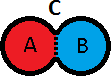
\includegraphics[width=0.075\textwidth]{fus.png} \hspace*{7cm}
        
\includegraphics[width=0.045\textwidth]{incorp.png} \hspace*{7cm}
        
\includegraphics[width=0.045\textwidth]{aquis.png} \hspace*{7cm}
        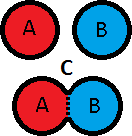
\includegraphics[width=0.075\textwidth]{jv.png}
        \end{center}
    \end{tikzfigure}
    \hspace*{6.75cm} \textbf{Fusão} \hspace*{7.45cm} \textbf{Incorporação} \hspace*{4.8cm} \textbf{Aquisição} \hspace*{6.05cm} \textbf{Joint Venture}

    }

    \block{Reconhecimento de Entidades Mencionadas}{
    Uma entidade mencionada (EM) é um objeto do mundo real que possui um nome próprio, como por exemplo uma pessoa ou uma organização. As entidades mencionadas do
    córpus foram anotadas por meio de uma ferramenta \textit{web} chamada BRAT [3], v.1.3.0, um projeto \textit{open source} (Licença MIT) recente, desenvolvido colaborativamente por
    pesquisadores de vários grupos distintos com interesse em anotações de texto. Na Figura 1 abaixo, anotações BRAT em uma sentença de um Ato de Concentração:


    \begin{tikzfigure}
        \hspace*{-0.5cm}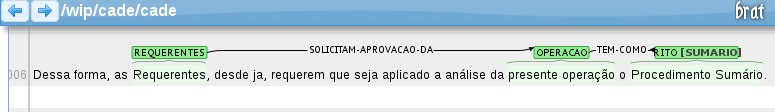
\includegraphics[width=0.6\textwidth]{bratposter.png}
    \end{tikzfigure}
    \begin{center}
      Figura 2: Anotações manuais de entidades mencionadas no BRAT de um dado Ato de Concentração.
    \end{center}

    Foram usados também os módulos de treinamento e reconhecimento de entidades mencionadas do Apache OpenNLP v.1.6.0 [4]. Na Figura 2, exemplo de saída
    de reconhecimento de entidades mencionadas de forma automatizada.

    \begin{tikzfigure}
        \hspace*{-0.5cm}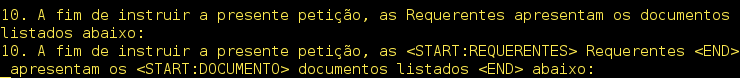
\includegraphics[width=0.615\textwidth]{opennlp.png}
    \end{tikzfigure}
    \begin{center}
      Figura 3: Reconhecimento de entidades mencionadas pelo Apache OpenNLP para a sentença dada.
    \end{center}
    }

    \block{Resultados}
    {
    Resultados da validação cruzada com o método \textit{holdout}. Cada $C_i$ representa uma combinação de grupos de teste e de treinamento compostos
    por cinco e quarenta e cinco Atos de Concentração, respectivamente. Os rótulos \textit{L} são apresentados na primeira coluna.

      \begin{center}
      \begin{tabular}{| P{5cm} | P{4cm} | P{4cm} | P{4cm} | P{4cm} | P{4cm} | P{4cm} | P{4cm} | P{4cm} | P{4cm} | P{4cm} |}
        \hline
        \backslashbox[45mm]{\textit{L}}{$C_i$} & $C_1$ & $C_2$ & $C_3$ & $C_4$ & $C_5$ & $C_6$ & $C_7$ & $C_8$ & $C_9$ & $C_{10}$ \\
        \hline
        \textbf{R}   & 327 & 263 & 218 & 324 & 293 & 210 & 270 & 263 & 220 & 243 \\ \hline
        \textbf{T}   & 774 & 527 & 491 & 741 & 653 & 520 & 702 & 623 & 587 & 605 \\ \hline
        \textbf{A}   & 258 & 208 & 168 & 248 & 231 & 162 & 208 & 210 & 179 & 184 \\ \hline
        \textbf{E1} + \textbf{E3} & 461 + 55 & 272 + 47 & 286 + 37 & 431 + 62 & 379 + 43 & 323 + 35 & 443 + 51 & 371 + 42 & 375 + 33 & 375 + 46 \\ \hline
        \textbf{E2} + \textbf{E3} & 14 + 55 & 8 + 47 & 13 + 37 & 14 + 62 & 19 + 43 & 13 + 35 & 11 + 51 & 11 + 42 & 8 + 33 & 13 + 46 \\ \hline\hline
        \textbf{P} & 0.789 & 0.790 & 0.770 & 0.765 & 0.788 & 0.771 & 0.770 & 0.798 & 0.813 & 0.757 \\ \hline
        \textbf{C} & 0.333 & 0.394 & 0.342 & 0.334 & 0.353 & 0.311 & 0.296 & 0.337 & 0.305 & 0.304 \\ \hline
        \textbf{F$_1$} & 0.468 & 0.525 & 0.473 & 0.465 & 0.487 & 0.443 & 0.427 & 0.473 & 0.443 & 0.433 \\ \hline
      \end{tabular}
      \end{center}

      \begin{center}
      \begin{tabular}{| l | l |}
        \arrayrulecolor{white}\hline
        R: & EMs recuperadas \\ \hline
        T: & EMs existentes na coleção \\ \hline
        A: & EMs corretamente recuperadas (VP) \\ \hline
      \end{tabular}
      \begin{tabular}{| l | l |}
        \arrayrulecolor{white}\hline
        E1: & EMs perdidas (FN) \\ \hline
        E2: & EMs classificadas erradas (FP) \\ \hline
        E3: & EMs imprecisas (FN e FP) \\ \hline
      \end{tabular}
      \begin{tabular}{| l | l |}
        \arrayrulecolor{white}\hline
        P: & Valor precisão \\ \hline
        C: & Valor cobertura \\ \hline
        F$_1$: & Valor medida-F balanceada \\ \hline
      \end{tabular}
      \end{center}
    }

    \block{Referências}
    {
      \begin{enumerate}[label={[\arabic*]}]
      \item Acesso à Informação: Conheça o CADE. Disponível em: $\langle$ http://www.cade.gov.br/acesso-a-informacao/institucional $\rangle$.
      \item MANNING, Christopher D., SCHUETZE, Hinrich. Foundations of Statistical Natural Language Processing, MIT Press. Cambridge, MA: May 1999.
      \item Pontus Stenetorp, Sampo Pyysalo, Goran Topić, Tomoko Ohta, Sophia Ananiadou and Jun'ichi Tsujii (2012). brat: a Web-based Tool for NLP-Assisted Text Annotation. In Proceedings of the Demonstrations Session at EACL 2012.
      \item Documentação Apache OpenNLP. Disponível em: $\langle$ https://opennlp.apache.org/documentation/1.6.0/manual/\newline opennlp.html $\rangle$.
      \item MANNING, Christopher D., RAGHAVAN, Prabhakar., SCHUETZE, Hinrich. An Introduction to Information Retrieval. Online Edition. Cambridge University Press. 2008.
      \end{enumerate}

      \vspace*{-0.25cm}
    }
\end{columns}

\end{document}

% https://pt.sharelatex.com/learn/Posters
